\section{The Hybrid Eulerian-Lagrangian Solver for the Vlasov system}
\label{sec:vlasov}
For the nonlinear resonant wave-particle interaction in weakly inhomogeneous magnetic field,
the  Hamiltonian 
 in the reference frames moving at local resonant velocities 
can be formulated in terms of   
the canonical variables $\xi,\Omega$ for the fast   varying
dynamics 
and $\vartheta,\mathcal{J}$ 
for the slowly varying scales
 \cite{zheng2023a}.
 Then the evolution of  perturbed distribution function $\delta f(\vartheta,\mathcal{J};\xi,\Omega;s,t)$ for the energetic particles is
\begin{equation}\label{eq.deltaf}
    \frac{\partial \delta f}{\partial t}+ \frac{d s}{d t} \frac{\partial \delta f}{\partial s} + \left[\delta f, H\right]_{\vartheta,\mathcal{J}} +  \left[\delta f, H\right]_{\xi,\Omega} = \mathcal{S}~,
\end{equation}
where $s$ is the distance along the magnetic field line and  the   Poisson brackets are defined as
\begin{equation}
    [f,~g]_{x,y} = \frac{\partial f}{\partial x}\frac{\partial g}{\partial y}-\frac{\partial f}{\partial y}\frac{\partial g}{\partial x}~.
\end{equation}
Here 
the source term $\mathcal{S}= -\left[f_0, \delta H\right]_{\vartheta, \mathcal{J}} - \left[f_0, \delta H\right]_{\xi, \Omega}$ 
where $f_0$ is the equilibrium distribution function and $\delta H$ denotes the perturbed Hamiltonian due to the resonant wave-particle interactions.
Note that the derivatives of $\delta H$ with respect to the slowly varying coordinates $\vartheta$ and $\mathcal{J}$ can be neglected due to the separation of perturbation and equilibrium scales. Besides, $\partial f_0/\partial \xi$ is vanished since $f_0$ does not generally depend on the fast varying angle coordinate $\xi$.
Thus, the source term can be simplified as 
\begin{equation}
     \mathcal{S} = \frac{\partial \delta H}{\partial \xi}\frac{\partial f_0}{\partial \Omega}.
\end{equation}
The variation of the angular coordinate $\vartheta$ is negligible due to the weakly inhomogeneous nature of the plasmas, while the dynamics of $\mathcal{J}, \Omega$, and $\xi$ remain entirely unaffected by $\vartheta$.
Therefore we neglect the term $ \dot{\vartheta} $ in the Vlasov equation and the  Poisson bracket becomes
\begin{equation}
\left[\delta f, H\right]_{\vartheta,\mathcal{J}}\simeq 
 -\dot{\mathcal{J}} \frac{\partial \delta f}{\partial \mathcal{J}}      
\end{equation}
where the dot denotes the time derivative.

We now implement the hybrid method to solve the Vlasov system, which has been structured to separate the fast and slowly varying scales within the Hamiltonian theory. We utilize the Eulerian method to model the fast-varying phase space $\xi,~\Omega$ and employ the Lagrangian method to model the slowly varying coordinates $\mathcal{J}$ and the resonance frame coordinate $s$.
The distribution function is written as \cite{shiroto2022}
\begin{equation}
    \delta f(\xi,\Omega,\mathcal{J},s,t) = \sum_{k,l} g_{k,l}(t,\xi,\Omega)\delta(s-s_k(t),\mathcal{J}-\mathcal{J}_l)~,
\end{equation}
where $g_{k,l}(t,\xi,\Omega)$ represents the distribution function in $\xi,\Omega$ space with $k$ and $l$ denoting the indices of the Lagrangian markers. 
Then the evolution equation for $g_{k,l}(t,\xi,\Omega)$ for each marker labeled by $k$ and $l$ is
\begin{equation}\label{eq.Euler}
\frac{\partial g}{\partial t} + \left[g,H\right]_{\xi,\Omega} = \mathcal{S}~.
\end{equation}
Here we omit the index $k$ and $l$ of $g$ for convenience.

In the Lagrangian step, it is essential for the marker to move  with the resonance frame throughout the spatial domain, i.e.,
\begin{equation}\label{eq.resonance}
        \dot{s}_k = v_r(s_k(t))~,
\end{equation}
where $v_r$ is  the  resonant velocity.
The motion equation for slowly varying coordinate $\mathcal{J}$ is
\begin{equation}
    \begin{aligned}\label{eq.Lagrangian}
        \dot{\mathcal{J}} &= \left[\mathcal{J},H\right]_{\vartheta,\mathcal{J}}~.
    \end{aligned}
\end{equation}

\subsection{The Eulerian step}
We first solve the fast-varying phase space dynamics for each Lagrangian marker at $s_k,\mathcal{J}_l$.
For the numerical treatment, the Vlasov equation (\ref{eq.Euler}) is expressed as
\begin{equation}\label{eq.Euler2}
    \frac{\partial g}{\partial t} + m \frac{\partial  g}{\partial \xi} - n \frac{\partial  g}{\partial \Omega}= \mathcal{S}~,
\end{equation}
where 
\begin{equation}
        m(\xi,\Omega) = \frac{\partial H}{\partial \Omega},~ n(\xi,\Omega) = \frac{\partial H}{\partial \xi}~.
\end{equation}
To achieve high-order accuracy, we apply the IDO method \cite{imadera2009} to solve the 2D Vlasov equation in $\xi,\Omega$ domain.
%The IDO scheme applies the polynomial as local interpolation functions to replace the distributions along each coordinate in phase space. 
% Here a second-order  polynomial is used as interpolation stencil for a function $g(x)$ from $x_i$ to $x_{i+1}$,
% \begin{equation}\label{eq.intg}
%     G(x,g_{i},g_{i+1},\sigma_{i+\frac{1}{2}}) = a\left(x-x_i\right)^2+b\left(x-x_i\right)+c~,
% \end{equation}
% where $g_i \equiv g(x_i)$, $g_{i+1} \equiv g(x_{i+1})$ are function values on the grid, and $\sigma_{i+\frac{1}{2}}$ is the cell integral value 
% \begin{equation}
%     \sigma_{i+\frac{1}{2}} \equiv \int_{x_i}^{x_{i+1}} g(x)~\mathrm{d}x~,
% \end{equation}
% and the coefficients are determined and from the grid value and the line integral over the cell,
% \begin{equation}
%     \begin{aligned}
%         a & =\frac{3\left(g_i+g_{i+1}\right)}{\Delta x^2}-\frac{6 \sigma_{i+\frac{1}{2}}}{\Delta x^3}~, \\
%         b & =-\frac{2\left(2 g_i+g_{i+1}\right)}{\Delta x}+\frac{6 \sigma_{i+\frac{1}{2}}}{\Delta x^2}~, \\
%         c & = g_i~.
%     \end{aligned}
% \end{equation}
%For equation (\ref{eq.Euler2}), 
The derivatives of $g$ with respect to $\xi$ and $\Omega$ are then approximated by 
the derivatives of 
a second-order  polynomial $G$ \cite{imadera2009}. 
%numerically represented by the interpolating stencil introduced above. 
The discretized form of the Vlasov equation (\ref{eq.Euler2}) becomes
\begin{equation}\label{eq.disV}
    \begin{aligned}
    \left.\frac{\partial g}{\partial t}\right|_{i,j}   & =  - m_{i,j} \left.\frac{\partial}{\partial \xi} G\left(\xi;g_{i,j},g_{i+1,j},\rho_{i+\frac{1}{2},j}\right)\right|_{i,j} 
    \\
    & + n_{i,j}  \left.\frac{\partial}{\partial \Omega}G\left(\Omega;g_{i,j},g_{i,j+1},\kappa_{i,j+\frac{1}{2}}\right)\right|_{i,j}
    \\
    & +  \mathcal{S}_{i,j}~,
    \end{aligned}
\end{equation}
where $G$ is a second-order  polynomial, $g_{i,j} $ are function values on the grid,  
$\rho_{i+\frac{1}{2},j}=\int_{\xi_i}^{\xi_{i+1}}g_{j}(\xi)\mathrm{d}\xi$ and $\kappa_{i,j+\frac{1}{2}}=\int_{\Omega_j}^{\Omega_{j+1}}g_{i}(\Omega)\mathrm{d}\Omega$
%$\rho_{i+\frac{1}{2},j}$ and $\kappa_{i,j+\frac{1}{2}}$ 
are the integrated function values over the grid.
Here $i$ and $j$ denote the grid index for $\xi$ and $\Omega$, respectively. 
The grid and interpolation are demonstrated in Fig.~\ref{fig.grids}.
\begin{figure}[htbp]
    \centering
    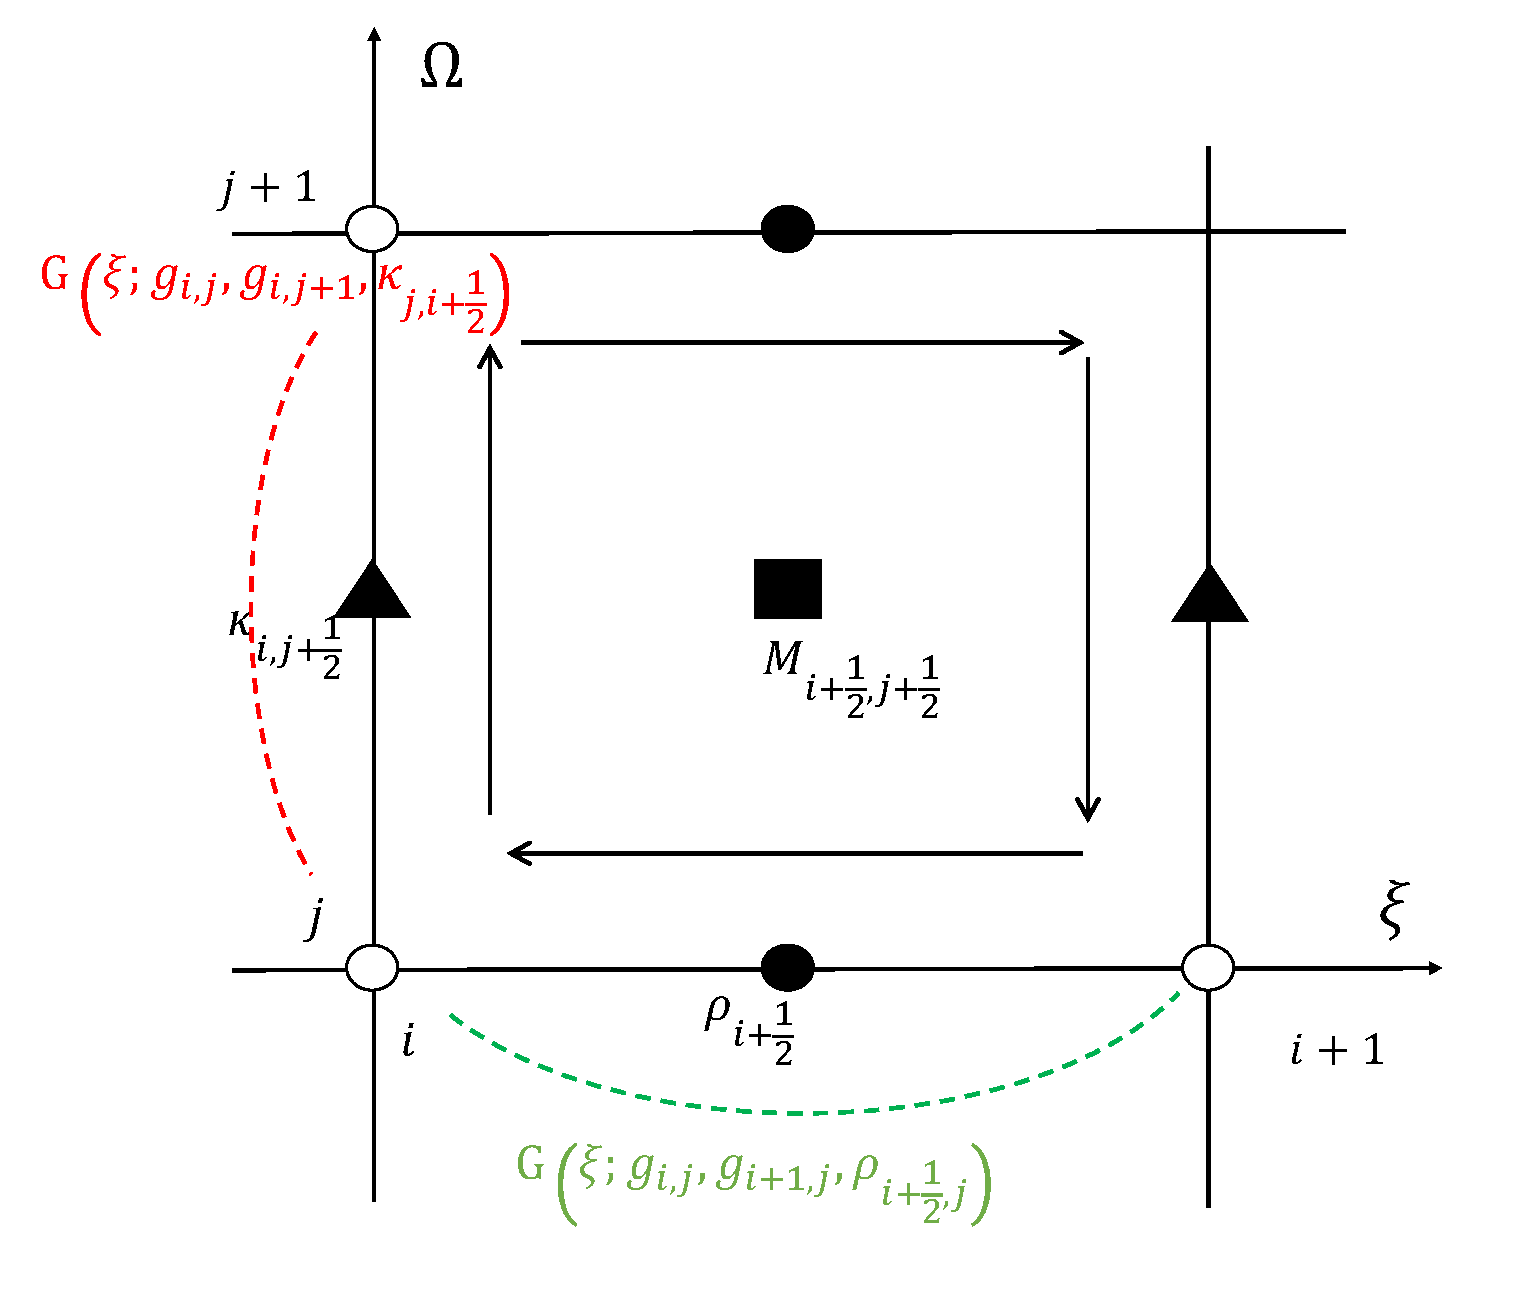
\includegraphics[scale=0.3]{cpc_img/IDO.pdf}
    \caption{The interpolating functions and  integrated values in $\xi,\Omega$ domain.}
    \label{fig.grids}
\end{figure}
%The interpolation relies on the line integrated values 
%The calculation at this step relies upon $\rho_{i+\frac{1}{2},j}$ and $\kappa_{i,j+\frac{1}{2}}$, which are the line integrated value of $\mathcal{F}$ 
%To solve the integral value $\rho$ and $\kappa$, we consider the  on given $j$ and $i$ grid respectively, and 
Integrating Eq.~(\ref{eq.Euler2}) along $\xi$ and $\Omega$ over the grid interval  yields the time evolution of the integral values \cite{imadera2009}
%, accroding to the definition in Eq.~(\ref{eq.intg}). The time evolution of the integral value is derived from the Vlasov equation,
\begin{equation}\label{eq.line}
    \begin{aligned}
    \left.\frac{\partial \rho}{\partial t}\right|_{i+\frac{1}{2},j} &= \int_{\xi_i}^{\xi_{i+1}}[ - m_j(\xi) \left.\frac{\partial g}{\partial \xi}\right|_{j}(\xi) + n_j(\xi) \left.\frac{\partial g}{\partial \Omega}\right|_{j}(\xi) + \mathcal{S}_j(\xi)]~\mathrm{d} \xi,
    \\
    \left.\frac{\partial \kappa}{\partial t}\right|_{i,j+\frac{1}{2}}
    &= \int_{\Omega_j}^{\Omega_{j+1}}[ - m_i(\Omega) \left.\frac{\partial g}{\partial \xi}\right|_{i}(\Omega) + n_i(\Omega) \left.\frac{\partial g}{\partial \Omega}\right|_{i}(\Omega) + \mathcal{S}_i(\Omega)]~\mathrm{d} \Omega.
    \end{aligned}
\end{equation}
%Then, enters step 2, solve Eq.~(\ref{eq.line})
%In the above integrals on the right-hand-side, We apply 
The third-order central interpolation scheme is applied to approximate the functions $m$ and $n$ along the $\xi$ and $\Omega$ dimension and the interpolating stencil is used to approximate the derivatives, 
\begin{equation}
    \begin{aligned}
       \left.\frac{\partial g}{\partial \xi}\right|_{j}(\xi)
        &\simeq G\left(\xi;\left.\frac{\partial g}{\partial \xi}\right|_{i,j},\left.\frac{\partial g}{\partial \xi}\right|_{i+1,j},g_{i+1,j}-g_{i,j}\right),
        \\
        \left.\frac{\partial g}{\partial \Omega}\right|_{j}(\xi)
         &\simeq G\left(\xi;\left.\frac{\partial g}{\partial \Omega}\right|_{i,j},\left.\frac{\partial g}{\partial \Omega}\right|_{i+1,j},    \left.\frac{\partial \rho}{\partial \Omega}\right|_{i+\frac{1}{2},j}\right),
         \\
         \left.\frac{\partial g}{\partial \Omega}\right|_{i}(\Omega) 
     &\simeq G\left(\Omega;\left.\frac{\partial g}{\partial \Omega}\right|_{i,j},\left.\frac{\partial g}{\partial \Omega}\right|_{i,j+1},g_{i,j+1}-g_{i,j}\right),\\
         \left.\frac{\partial g}{\partial \xi}\right|_{i}(\Omega) 
  &\simeq G\left(\Omega;\left.\frac{\partial g}{\partial \xi}\right|_{i,j},\left.\frac{\partial g}{\partial \xi}\right|_{i,j+1},\left.\frac{\partial \kappa}{\partial \xi}\right|_{i,j+\frac{1}{2}}\right),
    \end{aligned}
\end{equation}
%The interpolations bring new dependence on intergral value $\rho_{\Omega;i+\frac{1}{2},j}$ and $\kappa_{\xi;i,j+\frac{1}{2}}$. Therefore, 
%We apply additional interpolation functions to approximate 
%$\rho$ along $\Omega$ and $\kappa$ along $\xi$ to calculate its 
where 
%the derivatives
\begin{equation}
    \begin{aligned}
    \left.\frac{\partial \rho}{\partial \Omega}\right|_{i+\frac{1}{2},j}
    &\simeq \left.\frac{\partial}{\partial \Omega} G(\Omega;\rho_{i+\frac{1}{2},j},\rho_{i+\frac{1}{2},j+1}, M_{i+\frac{1}{2},j+\frac{1}{2}})\right|_{i+\frac{1}{2},j}~, \\
    \left.\frac{\partial \kappa}{\partial \xi}\right|_{i,j+\frac{1}{2}}
 &\simeq \left.\frac{\partial}{\partial \xi} G(\xi;\kappa_{i,j+\frac{1}{2}},\kappa_{i+1,j+\frac{1}{2}}, M_{i+\frac{1}{2},j+\frac{1}{2}})\right|_{i,j+\frac{1}{2}}~.
    \end{aligned}
\end{equation} 
%the interpolations rely both on 
%where the surface integral 
% and it can be readily transformed to the loop integral 
The time evolution of the surface integral $M_{i+\frac{1}{2},j+\frac{1}{2}}=\int_{\xi_i}^{\xi_{i+1}}\int_{\Omega_j}^{\Omega_{j+1}}g(t,\xi,\Omega)d\xi d\Omega$
% according to the Stokes theorem 
is given by \cite{imadera2009}
\begin{equation}\label{eq.area}
    \begin{aligned}
         \left.\frac{\partial M}{\partial t}\right|_{i+\frac{1}{2},j+\frac{1}{2}}
         &= \int_{\xi_i}^{\xi_{i+1}} n_{j+1}(\xi) g_{j+1}(\xi)~\mathrm{d}\xi - \int_{\Omega_j}^{\Omega_{j+1}} m_{i+1}(\Omega) g_{i+1} (\Omega)~\mathrm{d} \Omega \\
        & - \int_{\xi_i}^{\xi_{i+1}} n_{j}(\xi) g_{j}(\xi)~\mathrm{d}\xi + \int_{\Omega_j}^{\Omega_{j+1}} m_{i}(\Omega) g_{i} (\Omega) \mathrm{d}\Omega \\
        &+ \iint \mathcal{S}(\xi,\Omega)~\mathrm{d}\xi\mathrm{d}\Omega~,
    \end{aligned}
\end{equation}
where the integral of the source term is solved by trapezoidal integration.


Equations (\ref{eq.disV}), (\ref{eq.line}), and (\ref{eq.area})
are a set of ordinary differential equations that can be solved  by the RK method.
%-------------------------------%-------------------------------
For the boundary conditions, the values of the perturbed distribution vanish at the $\Omega$ boundaries
and
the distribution functions in  the resonant frame are assumed to be periodic in the  angle variable $\xi$,
\begin{equation}
    g\left(\xi,\Omega,t\right)=g\left(\xi+2 \pi,\Omega,t\right)~.
\end{equation}
Note that the periodic boundary conditions are valid only when the resonance does not deviate too far away from the  resonance frame of reference initially set in the simulation.



% \begin{figure}[htbp]
%     \centering
%     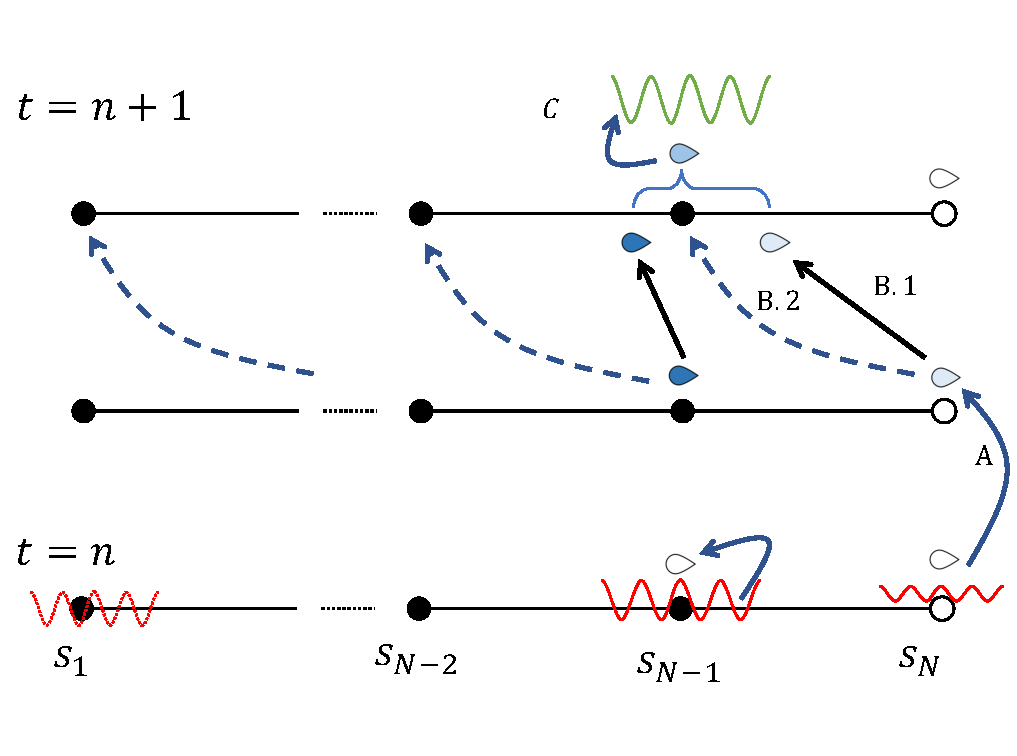
\includegraphics[scale=0.5]{cpc_img/Hybrid_demo.pdf}
%     \caption{Schematic illustration of the hybrid Vlasov simulation scheme.}
%     \label{fig.demo}
% \end{figure}

\subsection{The Lagrangian step}

To initially position the markers in the spatial domain, we place them on the fixed grid denoted as $s_k$.
%, which is the same grid used for solving the wave equations. 
To ensure that each marker updates over an identical time step, we implement nonuniform grid along the magnetic field line, as shown in Fig. \ref{fig.uni_grid}(a).
%, corresponding to the nonuniform wave grid. 
Initially, we calculate the transit time of a marker over the entire spatial domain,
\begin{equation}
    T = \int_{s_1}^{s_N} \frac{\mathrm{d}s}{v_r(s)}~,
\end{equation}
where $v_r(s)$ is the local resonant velocity that has been predetermined from the background equilibrium parameter.
Then the simulation time step is set as $\Delta t = T/N$ with $N$ the total number of sampling points/grids.
Finally, the initial spatial coordinates of the markers are set according to Eq. (\ref{eq.resonance}) which gives the trajectory of the marker,
\begin{equation}
    s_{k+1} = s_k +  \int_{t}^{t+\Delta t} v_r(s_k(t)) \mathrm{d}t~,
\end{equation}
where $k=1,2,3,...,N$.
%The nonuniform grids with size $\Delta s$ are 
Utilizing this nonuniform grid, the Lagrangian markers initially positioned on the grid advance to the next adjacent grid point after a time interval $\Delta t$.
\begin{figure}[htbp]
    \centering
    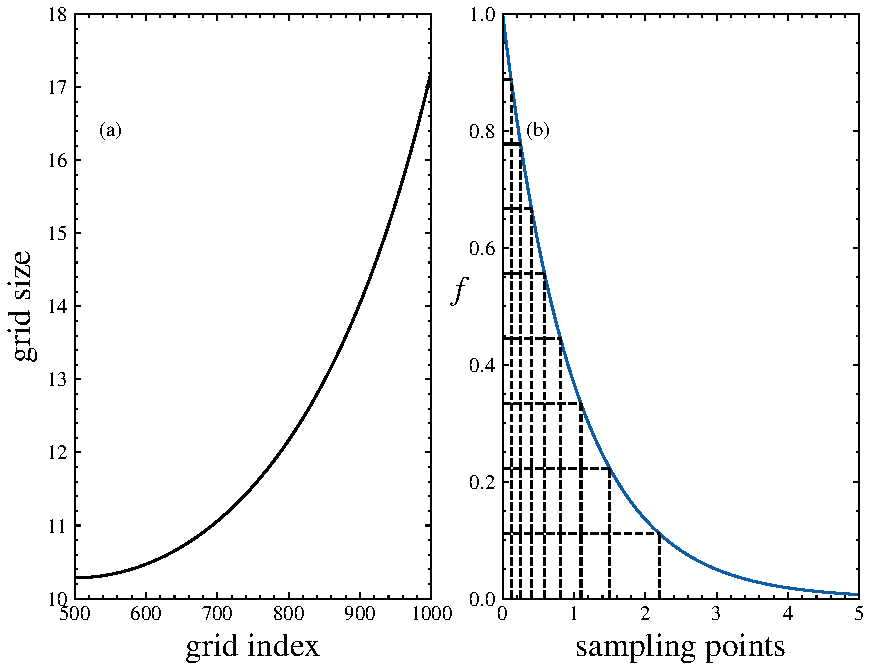
\includegraphics[scale=0.5]{cpc_img/fig_nu_grid.pdf}
    \caption{(a) Nonuniform spatial grid obtained from resonance velocity.
    (b) Sampling point for $\mathcal{J}$.
    %Here the number of grid points $N=500$.
    }
    \label{fig.uni_grid}
\end{figure}
Thus we successively push the distribution $g_{k,l}(\xi,\Omega)$  from  $s_k$ to the next grid $s_{k+1}$ for each time interval $\Delta t$.
After pushing the Lagrangian maker from the $n^\mathrm{th}$ to the $n+1^\mathrm{th}$ time step, the Hamiltonian  is re-calculated by  the  equilibrium quantities  at the new location of $s$ and $\mathcal{J}$, which are needed for evolving the distribution in $\xi-\Omega$ space at the next time step.

For the Lagrangian markers,
the sampling point for $\mathcal{J}$ is chosen to ensure  a uniform sampling to the initial equilibrium distribution $f_0$,
\begin{equation} 
    \mathcal{J}_l \to \int^{\mathcal{J}_l} f_0 \mathrm{d}\mathcal{J} = l/N~, 
\end{equation}
where $N$ is the total number of sampling points for $\mathcal{J}$. An illustration is shown in Fig. \ref{fig.uni_grid}(b).
The evolution of $\mathcal{J}$ in Eq. (\ref{eq.Lagrangian}) is simply solved by  the RK method.

\begin{figure}[htbp]
    \centering
    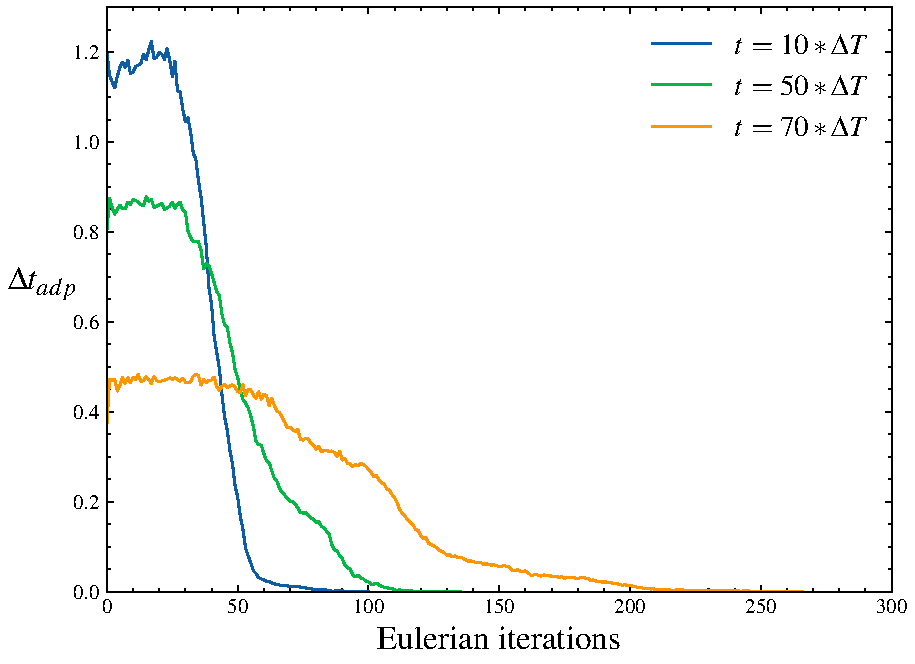
\includegraphics[scale=0.5]{cpc_img/fig_dts1.pdf}
    \caption{Variation of time step $\Delta t_\mathrm{adp}$ with the number of iterations for Eulerian calculation.  
    }
    \label{fig.adapetive}
\end{figure}
%Given that
Since the evolution in the $\xi,\Omega$  phase space 
is much 
%occurs at a significantly 
faster 
%pace compared to 
than that in the $s,\mathcal{J}$ domain, we employ a larger fixed time step $\Delta t$ for the Lagrangian calculations 
and a much smaller adaptive time step, $\Delta t_\mathrm{adp}$, for resolving the rapidly varying dynamics in the Eulerian domain. The time steps $\Delta t_\mathrm{adp}$ are adaptively determined through real-time error analysis using the adaptive RK method and satisfy
\begin{equation}
    \sum_{1}^N \Delta t_\mathrm{adp} = \Delta t ~,
\end{equation}
where $N$ is the total number of iterations within one $\Delta t$. 
As shown in Fig.~\ref{fig.adapetive}, 
$\Delta t_\mathrm{adp}$ is continuously adjusted and refined, consistently reducing its value whenever the numerical error exceeds the predefined error threshold. As the system undergoes nonlinear evolution, the time step $\Delta t_\mathrm{adp}$ undergoes further refinement, automatically increasing the number of iterations within a single $\Delta t$ interval. This highlights the clear advantage of adaptive hybrid methods in significantly improving computational efficiency.



%To mitigate the check board numerical error, 
Finally, we also implement a uniform grid and sample Lagrangian markers on $s$ to validate the effectiveness of our nonuniform grid approach.
After a given time step $\Delta t$ the markers deviated from the fixed grid, thus  we need to interpolate the distribution function and its derivatives required in the IDO scheme from the adjacent marker to the fixed $s$ grid.
These procedures closely resemble those of the semi-Lagrangian method \cite{sonnendrucker1999,cottet2018}. Following interpolation, the markers re-align with the grid, and the next iteration starts from the grid point.
As shown in Fig.~\ref{fig.cmp1}, the wave amplitudes calculated from  the two approaches converge  as the smaller grid sizes are used for the uniform grid with interpolation.  
\begin{figure}[htbp]
    \centering
    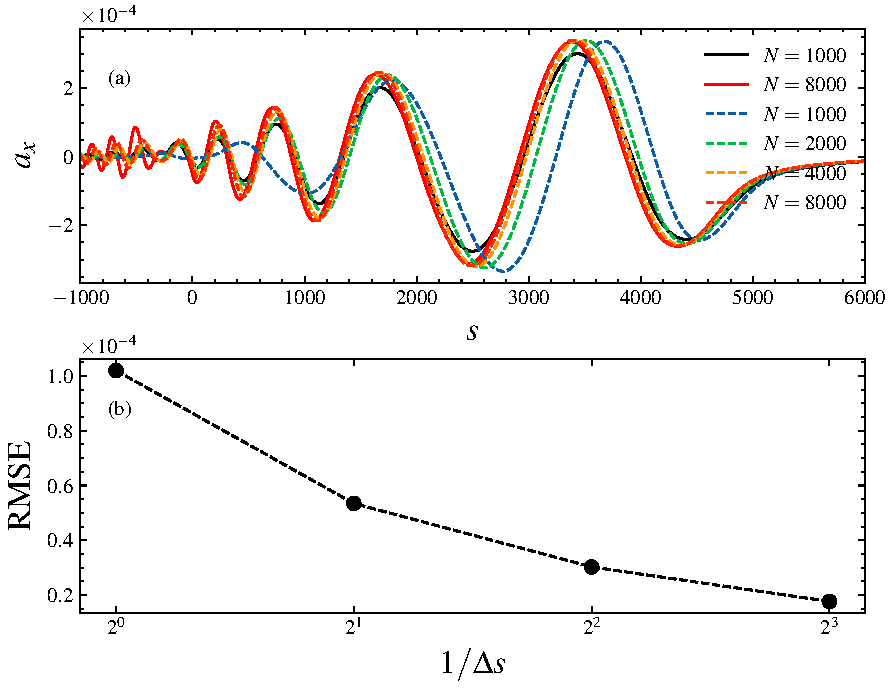
\includegraphics[scale=0.5]{cpc_img/fig_semiL.pdf}
    \caption{ (a) Wave amplitude from semi-Lagrangian method with linear interpolation of distribution at different uniform grid sizes (dashed-line) and the nonuniform grid (solid line).
    (b) Root-mean-square error at different uniform grid sizes compared to the 
    nonuniform grid of $N=8000$.
    }
    \label{fig.cmp1}
\end{figure}

